\documentclass[1p]{elsarticle_modified}
%\bibliographystyle{elsarticle-num}

%\usepackage[colorlinks]{hyperref}
%\usepackage{abbrmath_seonhwa} %\Abb, \Ascr, \Acal ,\Abf, \Afrak
\usepackage{amsfonts}
\usepackage{amssymb}
\usepackage{amsmath}
\usepackage{amsthm}
\usepackage{scalefnt}
\usepackage{amsbsy}
\usepackage{kotex}
\usepackage{caption}
\usepackage{subfig}
\usepackage{color}
\usepackage{graphicx}
\usepackage{xcolor} %% white, black, red, green, blue, cyan, magenta, yellow
\usepackage{float}
\usepackage{setspace}
\usepackage{hyperref}

\usepackage{tikz}
\usetikzlibrary{arrows}

\usepackage{multirow}
\usepackage{array} % fixed length table
\usepackage{hhline}

%%%%%%%%%%%%%%%%%%%%%
\makeatletter
\renewcommand*\env@matrix[1][\arraystretch]{%
	\edef\arraystretch{#1}%
	\hskip -\arraycolsep
	\let\@ifnextchar\new@ifnextchar
	\array{*\c@MaxMatrixCols c}}
\makeatother %https://tex.stackexchange.com/questions/14071/how-can-i-increase-the-line-spacing-in-a-matrix
%%%%%%%%%%%%%%%

\usepackage[normalem]{ulem}

\newcommand{\msout}[1]{\ifmmode\text{\sout{\ensuremath{#1}}}\else\sout{#1}\fi}
%SOURCE: \msout is \stkout macro in https://tex.stackexchange.com/questions/20609/strikeout-in-math-mode

\newcommand{\cancel}[1]{
	\ifmmode
	{\color{red}\msout{#1}}
	\else
	{\color{red}\sout{#1}}
	\fi
}

\newcommand{\add}[1]{
	{\color{blue}\uwave{#1}}
}

\newcommand{\replace}[2]{
	\ifmmode
	{\color{red}\msout{#1}}{\color{blue}\uwave{#2}}
	\else
	{\color{red}\sout{#1}}{\color{blue}\uwave{#2}}
	\fi
}

\newcommand{\Sol}{\mathcal{S}} %segment
\newcommand{\D}{D} %diagram
\newcommand{\A}{\mathcal{A}} %arc


%%%%%%%%%%%%%%%%%%%%%%%%%%%%%5 test

\def\sl{\operatorname{\textup{SL}}(2,\Cbb)}
\def\psl{\operatorname{\textup{PSL}}(2,\Cbb)}
\def\quan{\mkern 1mu \triangleright \mkern 1mu}

\theoremstyle{definition}
\newtheorem{thm}{Theorem}[section]
\newtheorem{prop}[thm]{Proposition}
\newtheorem{lem}[thm]{Lemma}
\newtheorem{ques}[thm]{Question}
\newtheorem{cor}[thm]{Corollary}
\newtheorem{defn}[thm]{Definition}
\newtheorem{exam}[thm]{Example}
\newtheorem{rmk}[thm]{Remark}
\newtheorem{alg}[thm]{Algorithm}

\newcommand{\I}{\sqrt{-1}}
\begin{document}

%\begin{frontmatter}
%
%\title{Boundary parabolic representations of knots up to 8 crossings}
%
%%% Group authors per affiliation:
%\author{Yunhi Cho} 
%\address{Department of Mathematics, University of Seoul, Seoul, Korea}
%\ead{yhcho@uos.ac.kr}
%
%
%\author{Seonhwa Kim} %\fnref{s_kim}}
%\address{Center for Geometry and Physics, Institute for Basic Science, Pohang, 37673, Korea}
%\ead{ryeona17@ibs.re.kr}
%
%\author{Hyuk Kim}
%\address{Department of Mathematical Sciences, Seoul National University, Seoul 08826, Korea}
%\ead{hyukkim@snu.ac.kr}
%
%\author{Seokbeom Yoon}
%\address{Department of Mathematical Sciences, Seoul National University, Seoul, 08826,  Korea}
%\ead{sbyoon15@snu.ac.kr}
%
%\begin{abstract}
%We find all boundary parabolic representation of knots up to 8 crossings.
%
%\end{abstract}
%\begin{keyword}
%    \MSC[2010] 57M25 
%\end{keyword}
%
%\end{frontmatter}

%\linenumbers
%\tableofcontents
%
\newcommand\colored[1]{\textcolor{white}{\rule[-0.35ex]{0.8em}{1.4ex}}\kern-0.8em\color{red} #1}%
%\newcommand\colored[1]{\textcolor{white}{ #1}\kern-2.17ex	\textcolor{white}{ #1}\kern-1.81ex	\textcolor{white}{ #1}\kern-2.15ex\color{red}#1	}

{\Large $\underline{12a_{0504}~(K12a_{0504})}$}

\setlength{\tabcolsep}{10pt}
\renewcommand{\arraystretch}{1.6}
\vspace{1cm}\begin{tabular}{m{100pt}>{\centering\arraybackslash}m{274pt}}
\multirow{5}{120pt}{
	\centering
	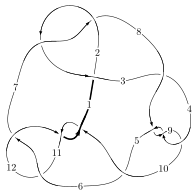
\includegraphics[width=112pt]{../../../GIT/diagram.site/Diagrams/png/1305_12a_0504.png}\\
\ \ \ A knot diagram\footnotemark}&
\allowdisplaybreaks
\textbf{Linearized knot diagam} \\
\cline{2-2}
 &
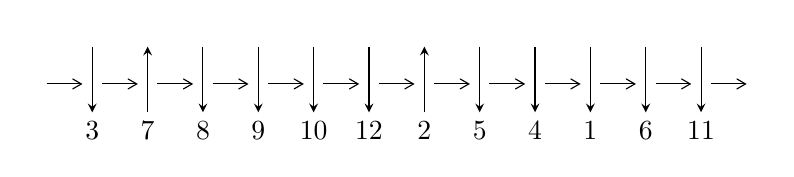
\begin{tikzpicture}[x=20pt, y=17pt]
	% nodes
	\node (C0) at (0, 0) {};
	\node (C1) at (1, 0) {};
	\node (C1U) at (1, +1) {};
	\node (C1D) at (1, -1) {3};

	\node (C2) at (2, 0) {};
	\node (C2U) at (2, +1) {};
	\node (C2D) at (2, -1) {7};

	\node (C3) at (3, 0) {};
	\node (C3U) at (3, +1) {};
	\node (C3D) at (3, -1) {8};

	\node (C4) at (4, 0) {};
	\node (C4U) at (4, +1) {};
	\node (C4D) at (4, -1) {9};

	\node (C5) at (5, 0) {};
	\node (C5U) at (5, +1) {};
	\node (C5D) at (5, -1) {10};

	\node (C6) at (6, 0) {};
	\node (C6U) at (6, +1) {};
	\node (C6D) at (6, -1) {12};

	\node (C7) at (7, 0) {};
	\node (C7U) at (7, +1) {};
	\node (C7D) at (7, -1) {2};

	\node (C8) at (8, 0) {};
	\node (C8U) at (8, +1) {};
	\node (C8D) at (8, -1) {5};

	\node (C9) at (9, 0) {};
	\node (C9U) at (9, +1) {};
	\node (C9D) at (9, -1) {4};

	\node (C10) at (10, 0) {};
	\node (C10U) at (10, +1) {};
	\node (C10D) at (10, -1) {1};

	\node (C11) at (11, 0) {};
	\node (C11U) at (11, +1) {};
	\node (C11D) at (11, -1) {6};

	\node (C12) at (12, 0) {};
	\node (C12U) at (12, +1) {};
	\node (C12D) at (12, -1) {11};
	\node (C13) at (13, 0) {};

	% arrows
	\draw[->,>={angle 60}]
	(C0) edge (C1) (C1) edge (C2) (C2) edge (C3) (C3) edge (C4) (C4) edge (C5) (C5) edge (C6) (C6) edge (C7) (C7) edge (C8) (C8) edge (C9) (C9) edge (C10) (C10) edge (C11) (C11) edge (C12) (C12) edge (C13) ;	\draw[->,>=stealth]
	(C1U) edge (C1D) (C2D) edge (C2U) (C3U) edge (C3D) (C4U) edge (C4D) (C5U) edge (C5D) (C6U) edge (C6D) (C7D) edge (C7U) (C8U) edge (C8D) (C9U) edge (C9D) (C10U) edge (C10D) (C11U) edge (C11D) (C12U) edge (C12D) ;
	\end{tikzpicture} \\
\hhline{~~} \\& 
\textbf{Solving Sequence} \\ \cline{2-2} 
 &
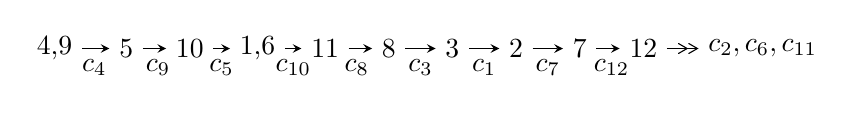
\begin{tikzpicture}[x=23pt, y=7pt]
	% node
	\node (A0) at (-1/8, 0) {4,9};
	\node (A1) at (1, 0) {5};
	\node (A2) at (2, 0) {10};
	\node (A3) at (49/16, 0) {1,6};
	\node (A4) at (33/8, 0) {11};
	\node (A5) at (41/8, 0) {8};
	\node (A6) at (49/8, 0) {3};
	\node (A7) at (57/8, 0) {2};
	\node (A8) at (65/8, 0) {7};
	\node (A9) at (73/8, 0) {12};
	\node (C1) at (1/2, -1) {$c_{4}$};
	\node (C2) at (3/2, -1) {$c_{9}$};
	\node (C3) at (5/2, -1) {$c_{5}$};
	\node (C4) at (29/8, -1) {$c_{10}$};
	\node (C5) at (37/8, -1) {$c_{8}$};
	\node (C6) at (45/8, -1) {$c_{3}$};
	\node (C7) at (53/8, -1) {$c_{1}$};
	\node (C8) at (61/8, -1) {$c_{7}$};
	\node (C9) at (69/8, -1) {$c_{12}$};
	\node (A10) at (11, 0) {$c_{2},c_{6},c_{11}$};

	% edge
	\draw[->,>=stealth]	
	(A0) edge (A1) (A1) edge (A2) (A2) edge (A3) (A3) edge (A4) (A4) edge (A5) (A5) edge (A6) (A6) edge (A7) (A7) edge (A8) (A8) edge (A9) ;
	\draw[->>,>={angle 60}]	
	(A9) edge (A10);
\end{tikzpicture} \\ 

\end{tabular} \\

\footnotetext{
The image of knot diagram is generated by the software ``\textbf{Draw programme}" developed by Andrew Bartholomew(\url{http://www.layer8.co.uk/maths/draw/index.htm\#Running-draw}), where we modified some parts for our purpose(\url{https://github.com/CATsTAILs/LinksPainter}).
}\phantom \\ \newline 
\centering \textbf{Ideals for irreducible components\footnotemark of $X_{\text{par}}$} 
 
\begin{align*}
I^u_{1}&=\langle 
-7.83895\times10^{14} u^{55}+1.45886\times10^{14} u^{54}+\cdots+3.67417\times10^{15} b-1.23817\times10^{16},\\
\phantom{I^u_{1}}&\phantom{= \langle  }9.64057\times10^{16} u^{55}-1.02861\times10^{17} u^{54}+\cdots+1.46967\times10^{16} a+5.86299\times10^{17},\;u^{56}- u^{55}+\cdots+12 u+1\rangle \\
I^u_{2}&=\langle 
- u^8-2 u^6-2 u^4+b,\;- u^6- u^4+a+1,\;u^{24}+8 u^{22}+\cdots+2 u-1\rangle \\
I^u_{3}&=\langle 
b+1,\;a^2- a u-2 a+u,\;u^2+1\rangle \\
\\
\end{align*}
\raggedright * 3 irreducible components of $\dim_{\mathbb{C}}=0$, with total 84 representations.\\
\footnotetext{All coefficients of polynomials are rational numbers. But the coefficients are sometimes approximated in decimal forms when there is not enough margin.}
\newpage
\renewcommand{\arraystretch}{1}
\centering \section*{I. $I^u_{1}= \langle -7.84\times10^{14} u^{55}+1.46\times10^{14} u^{54}+\cdots+3.67\times10^{15} b-1.24\times10^{16},\;9.64\times10^{16} u^{55}-1.03\times10^{17} u^{54}+\cdots+1.47\times10^{16} a+5.86\times10^{17},\;u^{56}- u^{55}+\cdots+12 u+1 \rangle$}
\flushleft \textbf{(i) Arc colorings}\\
\begin{tabular}{m{7pt} m{180pt} m{7pt} m{180pt} }
\flushright $a_{4}=$&$\begin{pmatrix}1\\0\end{pmatrix}$ \\
\flushright $a_{9}=$&$\begin{pmatrix}0\\u\end{pmatrix}$ \\
\flushright $a_{5}=$&$\begin{pmatrix}1\\u^2\end{pmatrix}$ \\
\flushright $a_{10}=$&$\begin{pmatrix}- u\\u\end{pmatrix}$ \\
\flushright $a_{1}=$&$\begin{pmatrix}-6.55969 u^{55}+6.99890 u^{54}+\cdots-234.424 u-39.8933\\0.213353 u^{55}-0.0397057 u^{54}+\cdots+14.8733 u+3.36993\end{pmatrix}$ \\
\flushright $a_{6}=$&$\begin{pmatrix}- u^4- u^2+1\\u^4+2 u^2\end{pmatrix}$ \\
\flushright $a_{11}=$&$\begin{pmatrix}-7.30147 u^{55}+8.14558 u^{54}+\cdots-237.184 u-48.1301\\-0.805092 u^{55}+0.773921 u^{54}+\cdots-22.7624 u-4.24178\end{pmatrix}$ \\
\flushright $a_{8}=$&$\begin{pmatrix}u\\u^3+u\end{pmatrix}$ \\
\flushright $a_{3}=$&$\begin{pmatrix}- u^4- u^2+1\\- u^6-2 u^4- u^2\end{pmatrix}$ \\
\flushright $a_{2}=$&$\begin{pmatrix}-6.66140 u^{55}+7.11337 u^{54}+\cdots-239.072 u-41.8370\\-0.0587147 u^{55}-0.0808551 u^{54}+\cdots+16.5555 u+3.49674\end{pmatrix}$ \\
\flushright $a_{7}=$&$\begin{pmatrix}-2.86544 u^{55}+2.88023 u^{54}+\cdots-100.769 u-25.4493\\-0.943701 u^{55}+1.04541 u^{54}+\cdots-36.4118 u-6.67618\end{pmatrix}$ \\
\flushright $a_{12}=$&$\begin{pmatrix}-6.53973 u^{55}+7.49680 u^{54}+\cdots-215.901 u-45.3003\\-1.08495 u^{55}+0.999699 u^{54}+\cdots-25.8687 u-4.36852\end{pmatrix}$\\&\end{tabular}
\flushleft \textbf{(ii) Obstruction class $= -1$}\\~\\
\flushleft \textbf{(iii) Cusp Shapes $= -\frac{14833210943177139}{3674173150903357} u^{55}+\frac{13598122062567921}{3674173150903357} u^{54}+\cdots-\frac{427855008730402692}{3674173150903357} u-\frac{136869864770758331}{3674173150903357}$}\\~\\
\newpage\renewcommand{\arraystretch}{1}
\flushleft \textbf{(iv) u-Polynomials at the component}\newline \\
\begin{tabular}{m{50pt}|m{274pt}}
Crossings & \hspace{64pt}u-Polynomials at each crossing \\
\hline $$\begin{aligned}c_{1}\end{aligned}$$&$\begin{aligned}
&u^{56}+29 u^{55}+\cdots+6 u+1
\end{aligned}$\\
\hline $$\begin{aligned}c_{2},c_{7}\end{aligned}$$&$\begin{aligned}
&u^{56}+u^{55}+\cdots-2 u+1
\end{aligned}$\\
\hline $$\begin{aligned}c_{3},c_{5}\end{aligned}$$&$\begin{aligned}
&u^{56}+2 u^{55}+\cdots-464 u+32
\end{aligned}$\\
\hline $$\begin{aligned}c_{4},c_{8},c_{9}\end{aligned}$$&$\begin{aligned}
&u^{56}+u^{55}+\cdots-12 u+1
\end{aligned}$\\
\hline $$\begin{aligned}c_{6},c_{11}\end{aligned}$$&$\begin{aligned}
&u^{56}-2 u^{55}+\cdots-3 u+2
\end{aligned}$\\
\hline $$\begin{aligned}c_{10},c_{12}\end{aligned}$$&$\begin{aligned}
&u^{56}+20 u^{55}+\cdots-19 u+4
\end{aligned}$\\
\hline
\end{tabular}\\~\\
\newpage\renewcommand{\arraystretch}{1}
\flushleft \textbf{(v) Riley Polynomials at the component}\newline \\
\begin{tabular}{m{50pt}|m{274pt}}
Crossings & \hspace{64pt}Riley Polynomials at each crossing \\
\hline $$\begin{aligned}c_{1}\end{aligned}$$&$\begin{aligned}
&y^{56}+y^{55}+\cdots+78 y+1
\end{aligned}$\\
\hline $$\begin{aligned}c_{2},c_{7}\end{aligned}$$&$\begin{aligned}
&y^{56}+29 y^{55}+\cdots+6 y+1
\end{aligned}$\\
\hline $$\begin{aligned}c_{3},c_{5}\end{aligned}$$&$\begin{aligned}
&y^{56}-42 y^{55}+\cdots-81664 y+1024
\end{aligned}$\\
\hline $$\begin{aligned}c_{4},c_{8},c_{9}\end{aligned}$$&$\begin{aligned}
&y^{56}+49 y^{55}+\cdots-90 y+1
\end{aligned}$\\
\hline $$\begin{aligned}c_{6},c_{11}\end{aligned}$$&$\begin{aligned}
&y^{56}-20 y^{55}+\cdots+19 y+4
\end{aligned}$\\
\hline $$\begin{aligned}c_{10},c_{12}\end{aligned}$$&$\begin{aligned}
&y^{56}+32 y^{55}+\cdots-33 y+16
\end{aligned}$\\
\hline
\end{tabular}\\~\\
\newpage\flushleft \textbf{(vi) Complex Volumes and Cusp Shapes}
$$\begin{array}{c|c|c}  
\text{Solutions to }I^u_{1}& \I (\text{vol} + \sqrt{-1}CS) & \text{Cusp shape}\\
 \hline 
\begin{aligned}
u &= \phantom{-}0.889558 + 0.109792 I \\
a &= \phantom{-}0.480562 - 0.208021 I \\
b &= -1.39404 - 1.26418 I\end{aligned}
 & -5.62716 - 11.26020 I & -12.2899 + 8.2594 I \\ \hline\begin{aligned}
u &= \phantom{-}0.889558 - 0.109792 I \\
a &= \phantom{-}0.480562 + 0.208021 I \\
b &= -1.39404 + 1.26418 I\end{aligned}
 & -5.62716 + 11.26020 I & -12.2899 - 8.2594 I \\ \hline\begin{aligned}
u &= \phantom{-}0.185587 + 0.860066 I \\
a &= -1.024400 + 0.085895 I \\
b &= -0.0405782 + 0.0105793 I\end{aligned}
 & \phantom{-}1.79150 - 2.20957 I & -3.12470 + 4.68768 I \\ \hline\begin{aligned}
u &= \phantom{-}0.185587 - 0.860066 I \\
a &= -1.024400 - 0.085895 I \\
b &= -0.0405782 - 0.0105793 I\end{aligned}
 & \phantom{-}1.79150 + 2.20957 I & -3.12470 - 4.68768 I \\ \hline\begin{aligned}
u &= -0.861042 + 0.114062 I \\
a &= \phantom{-}0.614579 + 0.107443 I \\
b &= -1.091830 + 0.875986 I\end{aligned}
 & -4.20562 + 5.74688 I & -10.33539 - 3.77278 I \\ \hline\begin{aligned}
u &= -0.861042 - 0.114062 I \\
a &= \phantom{-}0.614579 - 0.107443 I \\
b &= -1.091830 - 0.875986 I\end{aligned}
 & -4.20562 - 5.74688 I & -10.33539 + 3.77278 I \\ \hline\begin{aligned}
u &= \phantom{-}0.860629 + 0.049985 I \\
a &= \phantom{-}0.413499 + 0.208652 I \\
b &= -1.88213 - 0.20431 I\end{aligned}
 & -10.13050 - 4.55338 I & -16.9525 + 3.5771 I \\ \hline\begin{aligned}
u &= \phantom{-}0.860629 - 0.049985 I \\
a &= \phantom{-}0.413499 - 0.208652 I \\
b &= -1.88213 + 0.20431 I\end{aligned}
 & -10.13050 + 4.55338 I & -16.9525 - 3.5771 I \\ \hline\begin{aligned}
u &= \phantom{-}0.805415 + 0.008477 I \\
a &= \phantom{-}0.690320 - 0.645957 I \\
b &= -1.58304 - 0.97985 I\end{aligned}
 & -6.37248 - 2.26636 I & -13.85594 + 1.85600 I \\ \hline\begin{aligned}
u &= \phantom{-}0.805415 - 0.008477 I \\
a &= \phantom{-}0.690320 + 0.645957 I \\
b &= -1.58304 + 0.97985 I\end{aligned}
 & -6.37248 + 2.26636 I & -13.85594 - 1.85600 I\\
 \hline 
 \end{array}$$\newpage$$\begin{array}{c|c|c}  
\text{Solutions to }I^u_{1}& \I (\text{vol} + \sqrt{-1}CS) & \text{Cusp shape}\\
 \hline 
\begin{aligned}
u &= -0.348712 + 1.145540 I \\
a &= -1.46239 + 0.70535 I \\
b &= \phantom{-}0.639092 + 0.118002 I\end{aligned}
 & \phantom{-}0.79022 - 2.20219 I & \phantom{-0.000000 } 0 \\ \hline\begin{aligned}
u &= -0.348712 - 1.145540 I \\
a &= -1.46239 - 0.70535 I \\
b &= \phantom{-}0.639092 - 0.118002 I\end{aligned}
 & \phantom{-}0.79022 + 2.20219 I & \phantom{-0.000000 } 0 \\ \hline\begin{aligned}
u &= -0.787481 + 0.037354 I \\
a &= \phantom{-}0.799208 - 0.381112 I \\
b &= -1.144440 - 0.535672 I\end{aligned}
 & -4.76193 + 2.90653 I & -11.38592 - 3.37449 I \\ \hline\begin{aligned}
u &= -0.787481 - 0.037354 I \\
a &= \phantom{-}0.799208 + 0.381112 I \\
b &= -1.144440 + 0.535672 I\end{aligned}
 & -4.76193 - 2.90653 I & -11.38592 + 3.37449 I \\ \hline\begin{aligned}
u &= -0.020700 + 1.221230 I \\
a &= -0.733753 + 1.108360 I \\
b &= \phantom{-}0.060419 - 0.425354 I\end{aligned}
 & \phantom{-}1.78925 - 1.40742 I & \phantom{-0.000000 } 0 \\ \hline\begin{aligned}
u &= -0.020700 - 1.221230 I \\
a &= -0.733753 - 1.108360 I \\
b &= \phantom{-}0.060419 + 0.425354 I\end{aligned}
 & \phantom{-}1.78925 + 1.40742 I & \phantom{-0.000000 } 0 \\ \hline\begin{aligned}
u &= -0.638508 + 0.407850 I \\
a &= \phantom{-}0.739741 - 0.354164 I \\
b &= \phantom{-}0.589927 - 0.778722 I\end{aligned}
 & \phantom{-}1.25611 + 6.62961 I & -7.45851 - 9.59429 I \\ \hline\begin{aligned}
u &= -0.638508 - 0.407850 I \\
a &= \phantom{-}0.739741 + 0.354164 I \\
b &= \phantom{-}0.589927 + 0.778722 I\end{aligned}
 & \phantom{-}1.25611 - 6.62961 I & -7.45851 + 9.59429 I \\ \hline\begin{aligned}
u &= \phantom{-}0.273524 + 1.225730 I \\
a &= -0.725644 - 0.884759 I \\
b &= \phantom{-}0.356539 + 0.597946 I\end{aligned}
 & \phantom{-}2.31046 - 2.56681 I & \phantom{-0.000000 } 0 \\ \hline\begin{aligned}
u &= \phantom{-}0.273524 - 1.225730 I \\
a &= -0.725644 + 0.884759 I \\
b &= \phantom{-}0.356539 - 0.597946 I\end{aligned}
 & \phantom{-}2.31046 + 2.56681 I & \phantom{-0.000000 } 0\\
 \hline 
 \end{array}$$\newpage$$\begin{array}{c|c|c}  
\text{Solutions to }I^u_{1}& \I (\text{vol} + \sqrt{-1}CS) & \text{Cusp shape}\\
 \hline 
\begin{aligned}
u &= \phantom{-}0.577497 + 0.456433 I \\
a &= \phantom{-}0.431719 + 0.400148 I \\
b &= \phantom{-}0.359836 + 0.827641 I\end{aligned}
 & \phantom{-}1.72923 - 1.31419 I & -5.78155 + 3.99484 I \\ \hline\begin{aligned}
u &= \phantom{-}0.577497 - 0.456433 I \\
a &= \phantom{-}0.431719 - 0.400148 I \\
b &= \phantom{-}0.359836 - 0.827641 I\end{aligned}
 & \phantom{-}1.72923 + 1.31419 I & -5.78155 - 3.99484 I \\ \hline\begin{aligned}
u &= -0.142801 + 1.272040 I \\
a &= \phantom{-}0.036090 + 1.373970 I \\
b &= \phantom{-}0.474215 - 0.667513 I\end{aligned}
 & \phantom{-}0.98358 + 4.96048 I & \phantom{-0.000000 } 0 \\ \hline\begin{aligned}
u &= -0.142801 - 1.272040 I \\
a &= \phantom{-}0.036090 - 1.373970 I \\
b &= \phantom{-}0.474215 + 0.667513 I\end{aligned}
 & \phantom{-}0.98358 - 4.96048 I & \phantom{-0.000000 } 0 \\ \hline\begin{aligned}
u &= \phantom{-}0.354849 + 1.262830 I \\
a &= \phantom{-}1.64828 + 0.90921 I \\
b &= -0.868433 - 0.073319 I\end{aligned}
 & -2.48382 - 1.91013 I & \phantom{-0.000000 } 0 \\ \hline\begin{aligned}
u &= \phantom{-}0.354849 - 1.262830 I \\
a &= \phantom{-}1.64828 - 0.90921 I \\
b &= -0.868433 + 0.073319 I\end{aligned}
 & -2.48382 + 1.91013 I & \phantom{-0.000000 } 0 \\ \hline\begin{aligned}
u &= \phantom{-}0.058481 + 1.310540 I \\
a &= -0.153203 - 1.271200 I \\
b &= \phantom{-}0.086213 + 0.977970 I\end{aligned}
 & \phantom{-}4.34759 - 2.11198 I & \phantom{-0.000000 } 0 \\ \hline\begin{aligned}
u &= \phantom{-}0.058481 - 1.310540 I \\
a &= -0.153203 + 1.271200 I \\
b &= \phantom{-}0.086213 - 0.977970 I\end{aligned}
 & \phantom{-}4.34759 + 2.11198 I & \phantom{-0.000000 } 0 \\ \hline\begin{aligned}
u &= -0.366060 + 1.267250 I \\
a &= -1.13826 + 1.74843 I \\
b &= \phantom{-}1.48110 - 0.89517 I\end{aligned}
 & -2.57041 + 4.26504 I & \phantom{-0.000000 } 0 \\ \hline\begin{aligned}
u &= -0.366060 - 1.267250 I \\
a &= -1.13826 - 1.74843 I \\
b &= \phantom{-}1.48110 + 0.89517 I\end{aligned}
 & -2.57041 - 4.26504 I & \phantom{-0.000000 } 0\\
 \hline 
 \end{array}$$\newpage$$\begin{array}{c|c|c}  
\text{Solutions to }I^u_{1}& \I (\text{vol} + \sqrt{-1}CS) & \text{Cusp shape}\\
 \hline 
\begin{aligned}
u &= -0.346195 + 1.296780 I \\
a &= \phantom{-}0.98892 - 1.05718 I \\
b &= -0.612467 + 0.642893 I\end{aligned}
 & -0.59522 + 6.99644 I & \phantom{-0.000000 } 0 \\ \hline\begin{aligned}
u &= -0.346195 - 1.296780 I \\
a &= \phantom{-}0.98892 + 1.05718 I \\
b &= -0.612467 - 0.642893 I\end{aligned}
 & -0.59522 - 6.99644 I & \phantom{-0.000000 } 0 \\ \hline\begin{aligned}
u &= \phantom{-}0.390452 + 1.308290 I \\
a &= \phantom{-}1.15405 + 1.99315 I \\
b &= -1.52261 - 1.10872 I\end{aligned}
 & -5.88872 - 9.04102 I & \phantom{-0.000000 } 0 \\ \hline\begin{aligned}
u &= \phantom{-}0.390452 - 1.308290 I \\
a &= \phantom{-}1.15405 - 1.99315 I \\
b &= -1.52261 + 1.10872 I\end{aligned}
 & -5.88872 + 9.04102 I & \phantom{-0.000000 } 0 \\ \hline\begin{aligned}
u &= \phantom{-}0.335008 + 1.329430 I \\
a &= -0.32616 - 2.08418 I \\
b &= \phantom{-}1.05385 + 2.07205 I\end{aligned}
 & \phantom{-}3.44326 - 5.11122 I & \phantom{-0.000000 } 0 \\ \hline\begin{aligned}
u &= \phantom{-}0.335008 - 1.329430 I \\
a &= -0.32616 + 2.08418 I \\
b &= \phantom{-}1.05385 - 2.07205 I\end{aligned}
 & \phantom{-}3.44326 + 5.11122 I & \phantom{-0.000000 } 0 \\ \hline\begin{aligned}
u &= -0.359700 + 1.337340 I \\
a &= -0.49062 + 2.42131 I \\
b &= \phantom{-}1.59665 - 2.26221 I\end{aligned}
 & \phantom{-}2.15359 + 10.68620 I & \phantom{-0.000000 } 0 \\ \hline\begin{aligned}
u &= -0.359700 - 1.337340 I \\
a &= -0.49062 - 2.42131 I \\
b &= \phantom{-}1.59665 + 2.26221 I\end{aligned}
 & \phantom{-}2.15359 - 10.68620 I & \phantom{-0.000000 } 0 \\ \hline\begin{aligned}
u &= \phantom{-}0.102530 + 1.394500 I \\
a &= \phantom{-}0.964979 + 0.507457 I \\
b &= -1.93891 - 0.37473 I\end{aligned}
 & \phantom{-}8.29178 - 4.25641 I & \phantom{-0.000000 } 0 \\ \hline\begin{aligned}
u &= \phantom{-}0.102530 - 1.394500 I \\
a &= \phantom{-}0.964979 - 0.507457 I \\
b &= -1.93891 + 0.37473 I\end{aligned}
 & \phantom{-}8.29178 + 4.25641 I & \phantom{-0.000000 } 0\\
 \hline 
 \end{array}$$\newpage$$\begin{array}{c|c|c}  
\text{Solutions to }I^u_{1}& \I (\text{vol} + \sqrt{-1}CS) & \text{Cusp shape}\\
 \hline 
\begin{aligned}
u &= -0.066007 + 1.396890 I \\
a &= \phantom{-}0.810504 - 0.885178 I \\
b &= -1.69144 + 0.97965 I\end{aligned}
 & \phantom{-}8.59831 - 1.41502 I & \phantom{-0.000000 } 0 \\ \hline\begin{aligned}
u &= -0.066007 - 1.396890 I \\
a &= \phantom{-}0.810504 + 0.885178 I \\
b &= -1.69144 - 0.97965 I\end{aligned}
 & \phantom{-}8.59831 + 1.41502 I & \phantom{-0.000000 } 0 \\ \hline\begin{aligned}
u &= -0.381595 + 1.347340 I \\
a &= \phantom{-}0.25782 - 2.13685 I \\
b &= -0.98568 + 2.09120 I\end{aligned}
 & \phantom{-}0.38459 + 10.21060 I & \phantom{-0.000000 } 0 \\ \hline\begin{aligned}
u &= -0.381595 - 1.347340 I \\
a &= \phantom{-}0.25782 + 2.13685 I \\
b &= -0.98568 - 2.09120 I\end{aligned}
 & \phantom{-}0.38459 - 10.21060 I & \phantom{-0.000000 } 0 \\ \hline\begin{aligned}
u &= \phantom{-}0.149156 + 1.399160 I \\
a &= -0.56575 - 1.37488 I \\
b &= \phantom{-}1.40497 + 1.43686 I\end{aligned}
 & \phantom{-}7.66294 - 3.69333 I & \phantom{-0.000000 } 0 \\ \hline\begin{aligned}
u &= \phantom{-}0.149156 - 1.399160 I \\
a &= -0.56575 + 1.37488 I \\
b &= \phantom{-}1.40497 - 1.43686 I\end{aligned}
 & \phantom{-}7.66294 + 3.69333 I & \phantom{-0.000000 } 0 \\ \hline\begin{aligned}
u &= \phantom{-}0.397706 + 1.350820 I \\
a &= \phantom{-}0.30333 + 2.52636 I \\
b &= -1.42412 - 2.37758 I\end{aligned}
 & -1.0399 - 15.8746 I & \phantom{-0.000000 } 0 \\ \hline\begin{aligned}
u &= \phantom{-}0.397706 - 1.350820 I \\
a &= \phantom{-}0.30333 - 2.52636 I \\
b &= -1.42412 + 2.37758 I\end{aligned}
 & -1.0399 + 15.8746 I & \phantom{-0.000000 } 0 \\ \hline\begin{aligned}
u &= -0.181217 + 1.400850 I \\
a &= -0.752908 + 1.133180 I \\
b &= \phantom{-}1.76932 - 0.99764 I\end{aligned}
 & \phantom{-}7.06490 + 9.40242 I & \phantom{-0.000000 } 0 \\ \hline\begin{aligned}
u &= -0.181217 - 1.400850 I \\
a &= -0.752908 - 1.133180 I \\
b &= \phantom{-}1.76932 + 0.99764 I\end{aligned}
 & \phantom{-}7.06490 - 9.40242 I & \phantom{-0.000000 } 0\\
 \hline 
 \end{array}$$\newpage$$\begin{array}{c|c|c}  
\text{Solutions to }I^u_{1}& \I (\text{vol} + \sqrt{-1}CS) & \text{Cusp shape}\\
 \hline 
\begin{aligned}
u &= -0.502604 + 0.150960 I \\
a &= \phantom{-}1.119810 + 0.498449 I \\
b &= \phantom{-}0.406755 - 0.670085 I\end{aligned}
 & -3.33096 + 2.74558 I & -16.7867 - 5.9807 I \\ \hline\begin{aligned}
u &= -0.502604 - 0.150960 I \\
a &= \phantom{-}1.119810 - 0.498449 I \\
b &= \phantom{-}0.406755 + 0.670085 I\end{aligned}
 & -3.33096 - 2.74558 I & -16.7867 + 5.9807 I \\ \hline\begin{aligned}
u &= \phantom{-}0.268159 + 0.343396 I \\
a &= -0.410785 - 0.686556 I \\
b &= \phantom{-}0.387300 + 0.356715 I\end{aligned}
 & -0.578536 - 1.108330 I & -7.65763 + 5.69104 I \\ \hline\begin{aligned}
u &= \phantom{-}0.268159 - 0.343396 I \\
a &= -0.410785 + 0.686556 I \\
b &= \phantom{-}0.387300 - 0.356715 I\end{aligned}
 & -0.578536 + 1.108330 I & -7.65763 - 5.69104 I \\ \hline\begin{aligned}
u &= -0.145927 + 0.017514 I \\
a &= \phantom{-}3.33046 - 6.22037 I \\
b &= \phantom{-}1.013530 + 0.299730 I\end{aligned}
 & -1.72221 + 2.04047 I & -15.8987 - 3.0752 I \\ \hline\begin{aligned}
u &= -0.145927 - 0.017514 I \\
a &= \phantom{-}3.33046 + 6.22037 I \\
b &= \phantom{-}1.013530 - 0.299730 I\end{aligned}
 & -1.72221 - 2.04047 I & -15.8987 + 3.0752 I\\
 \hline 
 \end{array}$$\newpage\newpage\renewcommand{\arraystretch}{1}
\centering \section*{II. $I^u_{2}= \langle - u^8-2 u^6-2 u^4+b,\;- u^6- u^4+a+1,\;u^{24}+8 u^{22}+\cdots+2 u-1 \rangle$}
\flushleft \textbf{(i) Arc colorings}\\
\begin{tabular}{m{7pt} m{180pt} m{7pt} m{180pt} }
\flushright $a_{4}=$&$\begin{pmatrix}1\\0\end{pmatrix}$ \\
\flushright $a_{9}=$&$\begin{pmatrix}0\\u\end{pmatrix}$ \\
\flushright $a_{5}=$&$\begin{pmatrix}1\\u^2\end{pmatrix}$ \\
\flushright $a_{10}=$&$\begin{pmatrix}- u\\u\end{pmatrix}$ \\
\flushright $a_{1}=$&$\begin{pmatrix}u^6+u^4-1\\u^8+2 u^6+2 u^4\end{pmatrix}$ \\
\flushright $a_{6}=$&$\begin{pmatrix}- u^4- u^2+1\\u^4+2 u^2\end{pmatrix}$ \\
\flushright $a_{11}=$&$\begin{pmatrix}- u^{15}-4 u^{13}-6 u^{11}-2 u^9+4 u^7+4 u^5-2 u\\- u^{17}-5 u^{15}-11 u^{13}-12 u^{11}-5 u^9+2 u^7+2 u^5+u\end{pmatrix}$ \\
\flushright $a_{8}=$&$\begin{pmatrix}u\\u^3+u\end{pmatrix}$ \\
\flushright $a_{3}=$&$\begin{pmatrix}- u^4- u^2+1\\- u^6-2 u^4- u^2\end{pmatrix}$ \\
\flushright $a_{2}=$&$\begin{pmatrix}u^2-1\\u^4\end{pmatrix}$ \\
\flushright $a_{7}=$&$\begin{pmatrix}u^3\\u^5+u^3+u\end{pmatrix}$ \\
\flushright $a_{12}=$&$\begin{pmatrix}- u^{22}- u^{21}+\cdots-2 u^2-2 u\\- u^{23}+u^{22}+\cdots-2 u^3+2 u^2\end{pmatrix}$\\&\end{tabular}
\flushleft \textbf{(ii) Obstruction class $= -1$}\\~\\
\flushleft \textbf{(iii) Cusp Shapes $= -4 u^{18}-24 u^{16}-60 u^{14}-68 u^{12}-12 u^{10}-4 u^9+48 u^8-12 u^7+36 u^6-12 u^5-4 u^4+4 u^3-8 u^2+8 u-14$}\\~\\
\newpage\renewcommand{\arraystretch}{1}
\flushleft \textbf{(iv) u-Polynomials at the component}\newline \\
\begin{tabular}{m{50pt}|m{274pt}}
Crossings & \hspace{64pt}u-Polynomials at each crossing \\
\hline $$\begin{aligned}c_{1}\end{aligned}$$&$\begin{aligned}
&u^{24}+16 u^{23}+\cdots-4 u+1
\end{aligned}$\\
\hline $$\begin{aligned}c_{2},c_{4},c_{7}\\c_{8},c_{9}\end{aligned}$$&$\begin{aligned}
&u^{24}+8 u^{22}+\cdots-2 u-1
\end{aligned}$\\
\hline $$\begin{aligned}c_{3},c_{5}\end{aligned}$$&$\begin{aligned}
&(u^8- u^7-3 u^6+2 u^5+3 u^4-2 u-1)^3
\end{aligned}$\\
\hline $$\begin{aligned}c_{6},c_{11}\end{aligned}$$&$\begin{aligned}
&(u^8+u^7- u^6-2 u^5+u^4+2 u^3-2 u-1)^3
\end{aligned}$\\
\hline $$\begin{aligned}c_{10},c_{12}\end{aligned}$$&$\begin{aligned}
&(u^8+3 u^7+7 u^6+10 u^5+11 u^4+10 u^3+6 u^2+4 u+1)^3
\end{aligned}$\\
\hline
\end{tabular}\\~\\
\newpage\renewcommand{\arraystretch}{1}
\flushleft \textbf{(v) Riley Polynomials at the component}\newline \\
\begin{tabular}{m{50pt}|m{274pt}}
Crossings & \hspace{64pt}Riley Polynomials at each crossing \\
\hline $$\begin{aligned}c_{1}\end{aligned}$$&$\begin{aligned}
&y^{24}-16 y^{23}+\cdots-44 y+1
\end{aligned}$\\
\hline $$\begin{aligned}c_{2},c_{4},c_{7}\\c_{8},c_{9}\end{aligned}$$&$\begin{aligned}
&y^{24}+16 y^{23}+\cdots-4 y+1
\end{aligned}$\\
\hline $$\begin{aligned}c_{3},c_{5}\end{aligned}$$&$\begin{aligned}
&(y^8-7 y^7+19 y^6-22 y^5+3 y^4+14 y^3-6 y^2-4 y+1)^3
\end{aligned}$\\
\hline $$\begin{aligned}c_{6},c_{11}\end{aligned}$$&$\begin{aligned}
&(y^8-3 y^7+7 y^6-10 y^5+11 y^4-10 y^3+6 y^2-4 y+1)^3
\end{aligned}$\\
\hline $$\begin{aligned}c_{10},c_{12}\end{aligned}$$&$\begin{aligned}
&(y^8+5 y^7+11 y^6+6 y^5-17 y^4-34 y^3-22 y^2-4 y+1)^3
\end{aligned}$\\
\hline
\end{tabular}\\~\\
\newpage\flushleft \textbf{(vi) Complex Volumes and Cusp Shapes}
$$\begin{array}{c|c|c}  
\text{Solutions to }I^u_{2}& \I (\text{vol} + \sqrt{-1}CS) & \text{Cusp shape}\\
 \hline 
\begin{aligned}
u &= -0.199878 + 1.058230 I \\
a &= -0.692366 - 0.490639 I \\
b &= \phantom{-}0.755093 + 0.822738 I\end{aligned}
 & -0.845036\phantom{ +0.000000I} & -11.89446 + 0. I\phantom{ +0.000000I} \\ \hline\begin{aligned}
u &= -0.199878 - 1.058230 I \\
a &= -0.692366 + 0.490639 I \\
b &= \phantom{-}0.755093 - 0.822738 I\end{aligned}
 & -0.845036\phantom{ +0.000000I} & -11.89446 + 0. I\phantom{ +0.000000I} \\ \hline\begin{aligned}
u &= -0.817018 + 0.106623 I \\
a &= -0.377081 - 0.448378 I \\
b &= \phantom{-}1.35371 - 1.07975 I\end{aligned}
 & -2.37968 + 6.44354 I & -9.42845 - 5.29417 I \\ \hline\begin{aligned}
u &= -0.817018 - 0.106623 I \\
a &= -0.377081 + 0.448378 I \\
b &= \phantom{-}1.35371 + 1.07975 I\end{aligned}
 & -2.37968 - 6.44354 I & -9.42845 + 5.29417 I \\ \hline\begin{aligned}
u &= -0.819879\phantom{ +0.000000I} \\
a &= -0.244409\phantom{ +0.000000I} \\
b &= \phantom{-}1.71535\phantom{ +0.000000I}\end{aligned}
 & -6.50273\phantom{ +0.000000I} & -13.8640\phantom{ +0.000000I} \\ \hline\begin{aligned}
u &= -0.431691 + 0.692037 I \\
a &= -0.983121 + 0.409487 I \\
b &= -0.014801 + 0.629205 I\end{aligned}
 & \phantom{-}2.15941 - 2.57849 I & -4.27708 + 3.56796 I \\ \hline\begin{aligned}
u &= -0.431691 - 0.692037 I \\
a &= -0.983121 - 0.409487 I \\
b &= -0.014801 - 0.629205 I\end{aligned}
 & \phantom{-}2.15941 + 2.57849 I & -4.27708 - 3.56796 I \\ \hline\begin{aligned}
u &= -0.427601 + 1.146400 I \\
a &= \phantom{-}1.133070 - 0.604082 I \\
b &= -0.553659 + 0.206534 I\end{aligned}
 & -1.04066 - 1.13123 I & -7.41522 + 0.51079 I \\ \hline\begin{aligned}
u &= -0.427601 - 1.146400 I \\
a &= \phantom{-}1.133070 + 0.604082 I \\
b &= -0.553659 - 0.206534 I\end{aligned}
 & -1.04066 + 1.13123 I & -7.41522 - 0.51079 I \\ \hline\begin{aligned}
u &= \phantom{-}0.761196 + 0.098439 I \\
a &= -0.551326 + 0.313328 I \\
b &= \phantom{-}0.959472 + 0.729841 I\end{aligned}
 & -1.04066 - 1.13123 I & -7.41522 + 0.51079 I\\
 \hline 
 \end{array}$$\newpage$$\begin{array}{c|c|c}  
\text{Solutions to }I^u_{2}& \I (\text{vol} + \sqrt{-1}CS) & \text{Cusp shape}\\
 \hline 
\begin{aligned}
u &= \phantom{-}0.761196 - 0.098439 I \\
a &= -0.551326 - 0.313328 I \\
b &= \phantom{-}0.959472 - 0.729841 I\end{aligned}
 & -1.04066 + 1.13123 I & -7.41522 - 0.51079 I \\ \hline\begin{aligned}
u &= \phantom{-}0.461944 + 1.169380 I \\
a &= \phantom{-}1.66867 + 0.56200 I \\
b &= -0.853651 + 0.302978 I\end{aligned}
 & -2.37968 + 6.44354 I & -9.42845 - 5.29417 I \\ \hline\begin{aligned}
u &= \phantom{-}0.461944 - 1.169380 I \\
a &= \phantom{-}1.66867 - 0.56200 I \\
b &= -0.853651 - 0.302978 I\end{aligned}
 & -2.37968 - 6.44354 I & -9.42845 + 5.29417 I \\ \hline\begin{aligned}
u &= -0.028576 + 1.262710 I \\
a &= -2.48788 - 0.31944 I \\
b &= \phantom{-}3.39460 + 0.52702 I\end{aligned}
 & \phantom{-}2.15941 + 2.57849 I & -4.27708 - 3.56796 I \\ \hline\begin{aligned}
u &= -0.028576 - 1.262710 I \\
a &= -2.48788 + 0.31944 I \\
b &= \phantom{-}3.39460 - 0.52702 I\end{aligned}
 & \phantom{-}2.15941 - 2.57849 I & -4.27708 + 3.56796 I \\ \hline\begin{aligned}
u &= \phantom{-}0.460267 + 0.570674 I \\
a &= -1.170250 - 0.244142 I \\
b &= -0.285631 - 0.425378 I\end{aligned}
 & \phantom{-}2.15941 - 2.57849 I & -4.27708 + 3.56796 I \\ \hline\begin{aligned}
u &= \phantom{-}0.460267 - 0.570674 I \\
a &= -1.170250 + 0.244142 I \\
b &= -0.285631 + 0.425378 I\end{aligned}
 & \phantom{-}2.15941 + 2.57849 I & -4.27708 - 3.56796 I \\ \hline\begin{aligned}
u &= -0.333594 + 1.244840 I \\
a &= \phantom{-}0.37985 - 2.19261 I \\
b &= -1.04688 + 2.20428 I\end{aligned}
 & -1.04066 + 1.13123 I & -7.41522 - 0.51079 I \\ \hline\begin{aligned}
u &= -0.333594 - 1.244840 I \\
a &= \phantom{-}0.37985 + 2.19261 I \\
b &= -1.04688 - 2.20428 I\end{aligned}
 & -1.04066 - 1.13123 I & -7.41522 + 0.51079 I \\ \hline\begin{aligned}
u &= \phantom{-}0.409939 + 1.226440 I \\
a &= \phantom{-}1.44167 + 1.68145 I \\
b &= -1.73732 - 0.79694 I\end{aligned}
 & -6.50273\phantom{ +0.000000I} & -13.86404 + 0. I\phantom{ +0.000000I}\\
 \hline 
 \end{array}$$\newpage$$\begin{array}{c|c|c}  
\text{Solutions to }I^u_{2}& \I (\text{vol} + \sqrt{-1}CS) & \text{Cusp shape}\\
 \hline 
\begin{aligned}
u &= \phantom{-}0.409939 - 1.226440 I \\
a &= \phantom{-}1.44167 - 1.68145 I \\
b &= -1.73732 + 0.79694 I\end{aligned}
 & -6.50273\phantom{ +0.000000I} & -13.86404 + 0. I\phantom{ +0.000000I} \\ \hline\begin{aligned}
u &= \phantom{-}0.355074 + 1.276000 I \\
a &= \phantom{-}0.74615 + 2.66734 I \\
b &= -1.85855 - 2.47925 I\end{aligned}
 & -2.37968 - 6.44354 I & -9.42845 + 5.29417 I \\ \hline\begin{aligned}
u &= \phantom{-}0.355074 - 1.276000 I \\
a &= \phantom{-}0.74615 - 2.66734 I \\
b &= -1.85855 + 2.47925 I\end{aligned}
 & -2.37968 + 6.44354 I & -9.42845 - 5.29417 I \\ \hline\begin{aligned}
u &= \phantom{-}0.399757\phantom{ +0.000000I} \\
a &= -0.970381\phantom{ +0.000000I} \\
b &= \phantom{-}0.0598901\phantom{ +0.000000I}\end{aligned}
 & -0.845036\phantom{ +0.000000I} & -11.8940\phantom{ +0.000000I}\\
 \hline 
 \end{array}$$\newpage\newpage\renewcommand{\arraystretch}{1}
\centering \section*{III. $I^u_{3}= \langle b+1,\;a^2- a u-2 a+u,\;u^2+1 \rangle$}
\flushleft \textbf{(i) Arc colorings}\\
\begin{tabular}{m{7pt} m{180pt} m{7pt} m{180pt} }
\flushright $a_{4}=$&$\begin{pmatrix}1\\0\end{pmatrix}$ \\
\flushright $a_{9}=$&$\begin{pmatrix}0\\u\end{pmatrix}$ \\
\flushright $a_{5}=$&$\begin{pmatrix}1\\-1\end{pmatrix}$ \\
\flushright $a_{10}=$&$\begin{pmatrix}- u\\u\end{pmatrix}$ \\
\flushright $a_{1}=$&$\begin{pmatrix}a\\-1\end{pmatrix}$ \\
\flushright $a_{6}=$&$\begin{pmatrix}1\\-1\end{pmatrix}$ \\
\flushright $a_{11}=$&$\begin{pmatrix}- a u+a- u-1\\a u\end{pmatrix}$ \\
\flushright $a_{8}=$&$\begin{pmatrix}u\\0\end{pmatrix}$ \\
\flushright $a_{3}=$&$\begin{pmatrix}1\\0\end{pmatrix}$ \\
\flushright $a_{2}=$&$\begin{pmatrix}a+1\\-1\end{pmatrix}$ \\
\flushright $a_{7}=$&$\begin{pmatrix}- a u\\u\end{pmatrix}$ \\
\flushright $a_{12}=$&$\begin{pmatrix}- a u\\a u+a- u-1\end{pmatrix}$\\&\end{tabular}
\flushleft \textbf{(ii) Obstruction class $= 1$}\\~\\
\flushleft \textbf{(iii) Cusp Shapes $= -4 a u+4 u-12$}\\~\\
\newpage\renewcommand{\arraystretch}{1}
\flushleft \textbf{(iv) u-Polynomials at the component}\newline \\
\begin{tabular}{m{50pt}|m{274pt}}
Crossings & \hspace{64pt}u-Polynomials at each crossing \\
\hline $$\begin{aligned}c_{1}\end{aligned}$$&$\begin{aligned}
&(u-1)^4
\end{aligned}$\\
\hline $$\begin{aligned}c_{2},c_{4},c_{7}\\c_{8},c_{9}\end{aligned}$$&$\begin{aligned}
&(u^2+1)^2
\end{aligned}$\\
\hline $$\begin{aligned}c_{3},c_{5}\end{aligned}$$&$\begin{aligned}
&u^4
\end{aligned}$\\
\hline $$\begin{aligned}c_{6},c_{11}\end{aligned}$$&$\begin{aligned}
&u^4- u^2+1
\end{aligned}$\\
\hline $$\begin{aligned}c_{10}\end{aligned}$$&$\begin{aligned}
&(u^2- u+1)^2
\end{aligned}$\\
\hline $$\begin{aligned}c_{12}\end{aligned}$$&$\begin{aligned}
&(u^2+u+1)^2
\end{aligned}$\\
\hline
\end{tabular}\\~\\
\newpage\renewcommand{\arraystretch}{1}
\flushleft \textbf{(v) Riley Polynomials at the component}\newline \\
\begin{tabular}{m{50pt}|m{274pt}}
Crossings & \hspace{64pt}Riley Polynomials at each crossing \\
\hline $$\begin{aligned}c_{1}\end{aligned}$$&$\begin{aligned}
&(y-1)^4
\end{aligned}$\\
\hline $$\begin{aligned}c_{2},c_{4},c_{7}\\c_{8},c_{9}\end{aligned}$$&$\begin{aligned}
&(y+1)^4
\end{aligned}$\\
\hline $$\begin{aligned}c_{3},c_{5}\end{aligned}$$&$\begin{aligned}
&y^4
\end{aligned}$\\
\hline $$\begin{aligned}c_{6},c_{11}\end{aligned}$$&$\begin{aligned}
&(y^2- y+1)^2
\end{aligned}$\\
\hline $$\begin{aligned}c_{10},c_{12}\end{aligned}$$&$\begin{aligned}
&(y^2+y+1)^2
\end{aligned}$\\
\hline
\end{tabular}\\~\\
\newpage\flushleft \textbf{(vi) Complex Volumes and Cusp Shapes}
$$\begin{array}{c|c|c}  
\text{Solutions to }I^u_{3}& \I (\text{vol} + \sqrt{-1}CS) & \text{Cusp shape}\\
 \hline 
\begin{aligned}
u &= \phantom{-0.000000 -}1.000000 I \\
a &= \phantom{-}0.133975 + 0.500000 I \\
b &= -1.00000\phantom{ +0.000000I}\end{aligned}
 & \phantom{-0.000000 } -2.02988 I & -10.00000 + 3.46410 I \\ \hline\begin{aligned}
u &= \phantom{-0.000000 -}1.000000 I \\
a &= \phantom{-}1.86603 + 0.50000 I \\
b &= -1.00000\phantom{ +0.000000I}\end{aligned}
 & \phantom{-0.000000 -}2.02988 I & -10.00000 - 3.46410 I \\ \hline\begin{aligned}
u &= \phantom{-0.000000 } -1.000000 I \\
a &= \phantom{-}0.133975 - 0.500000 I \\
b &= -1.00000\phantom{ +0.000000I}\end{aligned}
 & \phantom{-0.000000 -}2.02988 I & -10.00000 - 3.46410 I \\ \hline\begin{aligned}
u &= \phantom{-0.000000 } -1.000000 I \\
a &= \phantom{-}1.86603 - 0.50000 I \\
b &= -1.00000\phantom{ +0.000000I}\end{aligned}
 & \phantom{-0.000000 } -2.02988 I & -10.00000 + 3.46410 I\\
 \hline 
 \end{array}$$\newpage
\newpage\renewcommand{\arraystretch}{1}
\centering \section*{ IV. u-Polynomials}
\begin{tabular}{m{50pt}|m{274pt}}
Crossings & \hspace{64pt}u-Polynomials at each crossing \\
\hline $$\begin{aligned}c_{1}\end{aligned}$$&$\begin{aligned}
&((u-1)^4)(u^{24}+16 u^{23}+\cdots-4 u+1)(u^{56}+29 u^{55}+\cdots+6 u+1)
\end{aligned}$\\
\hline $$\begin{aligned}c_{2},c_{7}\end{aligned}$$&$\begin{aligned}
&((u^2+1)^2)(u^{24}+8 u^{22}+\cdots-2 u-1)(u^{56}+u^{55}+\cdots-2 u+1)
\end{aligned}$\\
\hline $$\begin{aligned}c_{3},c_{5}\end{aligned}$$&$\begin{aligned}
&u^4(u^8- u^7+\cdots-2 u-1)^{3}(u^{56}+2 u^{55}+\cdots-464 u+32)
\end{aligned}$\\
\hline $$\begin{aligned}c_{4},c_{8},c_{9}\end{aligned}$$&$\begin{aligned}
&((u^2+1)^2)(u^{24}+8 u^{22}+\cdots-2 u-1)(u^{56}+u^{55}+\cdots-12 u+1)
\end{aligned}$\\
\hline $$\begin{aligned}c_{6},c_{11}\end{aligned}$$&$\begin{aligned}
&(u^4- u^2+1)(u^8+u^7- u^6-2 u^5+u^4+2 u^3-2 u-1)^3\\
&\cdot(u^{56}-2 u^{55}+\cdots-3 u+2)
\end{aligned}$\\
\hline $$\begin{aligned}c_{10}\end{aligned}$$&$\begin{aligned}
&(u^2- u+1)^2(u^8+3 u^7+7 u^6+10 u^5+11 u^4+10 u^3+6 u^2+4 u+1)^3\\
&\cdot(u^{56}+20 u^{55}+\cdots-19 u+4)
\end{aligned}$\\
\hline $$\begin{aligned}c_{12}\end{aligned}$$&$\begin{aligned}
&(u^2+u+1)^2(u^8+3 u^7+7 u^6+10 u^5+11 u^4+10 u^3+6 u^2+4 u+1)^3\\
&\cdot(u^{56}+20 u^{55}+\cdots-19 u+4)
\end{aligned}$\\
\hline
\end{tabular}\newpage\renewcommand{\arraystretch}{1}
\centering \section*{ V. Riley Polynomials}
\begin{tabular}{m{50pt}|m{274pt}}
Crossings & \hspace{64pt}Riley Polynomials at each crossing \\
\hline $$\begin{aligned}c_{1}\end{aligned}$$&$\begin{aligned}
&((y-1)^4)(y^{24}-16 y^{23}+\cdots-44 y+1)(y^{56}+y^{55}+\cdots+78 y+1)
\end{aligned}$\\
\hline $$\begin{aligned}c_{2},c_{7}\end{aligned}$$&$\begin{aligned}
&((y+1)^4)(y^{24}+16 y^{23}+\cdots-4 y+1)(y^{56}+29 y^{55}+\cdots+6 y+1)
\end{aligned}$\\
\hline $$\begin{aligned}c_{3},c_{5}\end{aligned}$$&$\begin{aligned}
&y^4(y^8-7 y^7+19 y^6-22 y^5+3 y^4+14 y^3-6 y^2-4 y+1)^3\\
&\cdot(y^{56}-42 y^{55}+\cdots-81664 y+1024)
\end{aligned}$\\
\hline $$\begin{aligned}c_{4},c_{8},c_{9}\end{aligned}$$&$\begin{aligned}
&((y+1)^4)(y^{24}+16 y^{23}+\cdots-4 y+1)(y^{56}+49 y^{55}+\cdots-90 y+1)
\end{aligned}$\\
\hline $$\begin{aligned}c_{6},c_{11}\end{aligned}$$&$\begin{aligned}
&(y^2- y+1)^2(y^8-3 y^7+7 y^6-10 y^5+11 y^4-10 y^3+6 y^2-4 y+1)^3\\
&\cdot(y^{56}-20 y^{55}+\cdots+19 y+4)
\end{aligned}$\\
\hline $$\begin{aligned}c_{10},c_{12}\end{aligned}$$&$\begin{aligned}
&(y^2+y+1)^2\\
&\cdot(y^8+5 y^7+11 y^6+6 y^5-17 y^4-34 y^3-22 y^2-4 y+1)^3\\
&\cdot(y^{56}+32 y^{55}+\cdots-33 y+16)
\end{aligned}$\\
\hline
\end{tabular}
\vskip 2pc
\end{document}